%% ============================================================
%% Chapter 6 — Results
%% ============================================================
\chapter{Results}
\label{chap:results}

\section{Strategy Comparison on the Test Set}
\label{sec:results_comparison}

Table~\ref{tab:strategy_comparison} summarises the performance of all three
strategies on the held-out test set of 1,200 questions. All hyper-parameters
were fixed prior to evaluation using the validation set only.

\begin{table}[htbp]
  \centering
  \caption{Abstention strategy comparison on the test set
           (1,200 questions: 600 answerable, 600 unanswerable).}
  \label{tab:strategy_comparison}
  \begin{tabular}{lcccccc}
    \toprule
    \textbf{Strategy} &
    \textbf{Precision} & \textbf{Recall} & \textbf{F1} &
    \textbf{Coverage} & \textbf{FAR} & \textbf{FAbR} \\
    \midrule
    Always Answer               & 0.4820 & 1.0000 & 0.6505 & 1.000 & 1.0000 & 0.0000 \\
    BM25 Threshold              & 0.4810 & 0.9959 & 0.6486 & 0.998 & 1.0000 & 0.0042 \\
    Answerability Classifier    & \textbf{0.8231} & 0.8880 & \textbf{0.8543} & 0.520 & \textbf{0.1776} & 0.1120 \\
    \bottomrule
    \multicolumn{7}{l}{\small FAR = False-Answer Rate; FAbR = False-Abstention Rate.} \\
    \multicolumn{7}{l}{\small Bold = best value in column.} \\
  \end{tabular}
\end{table}

\begin{figure}[htbp]
  \centering
  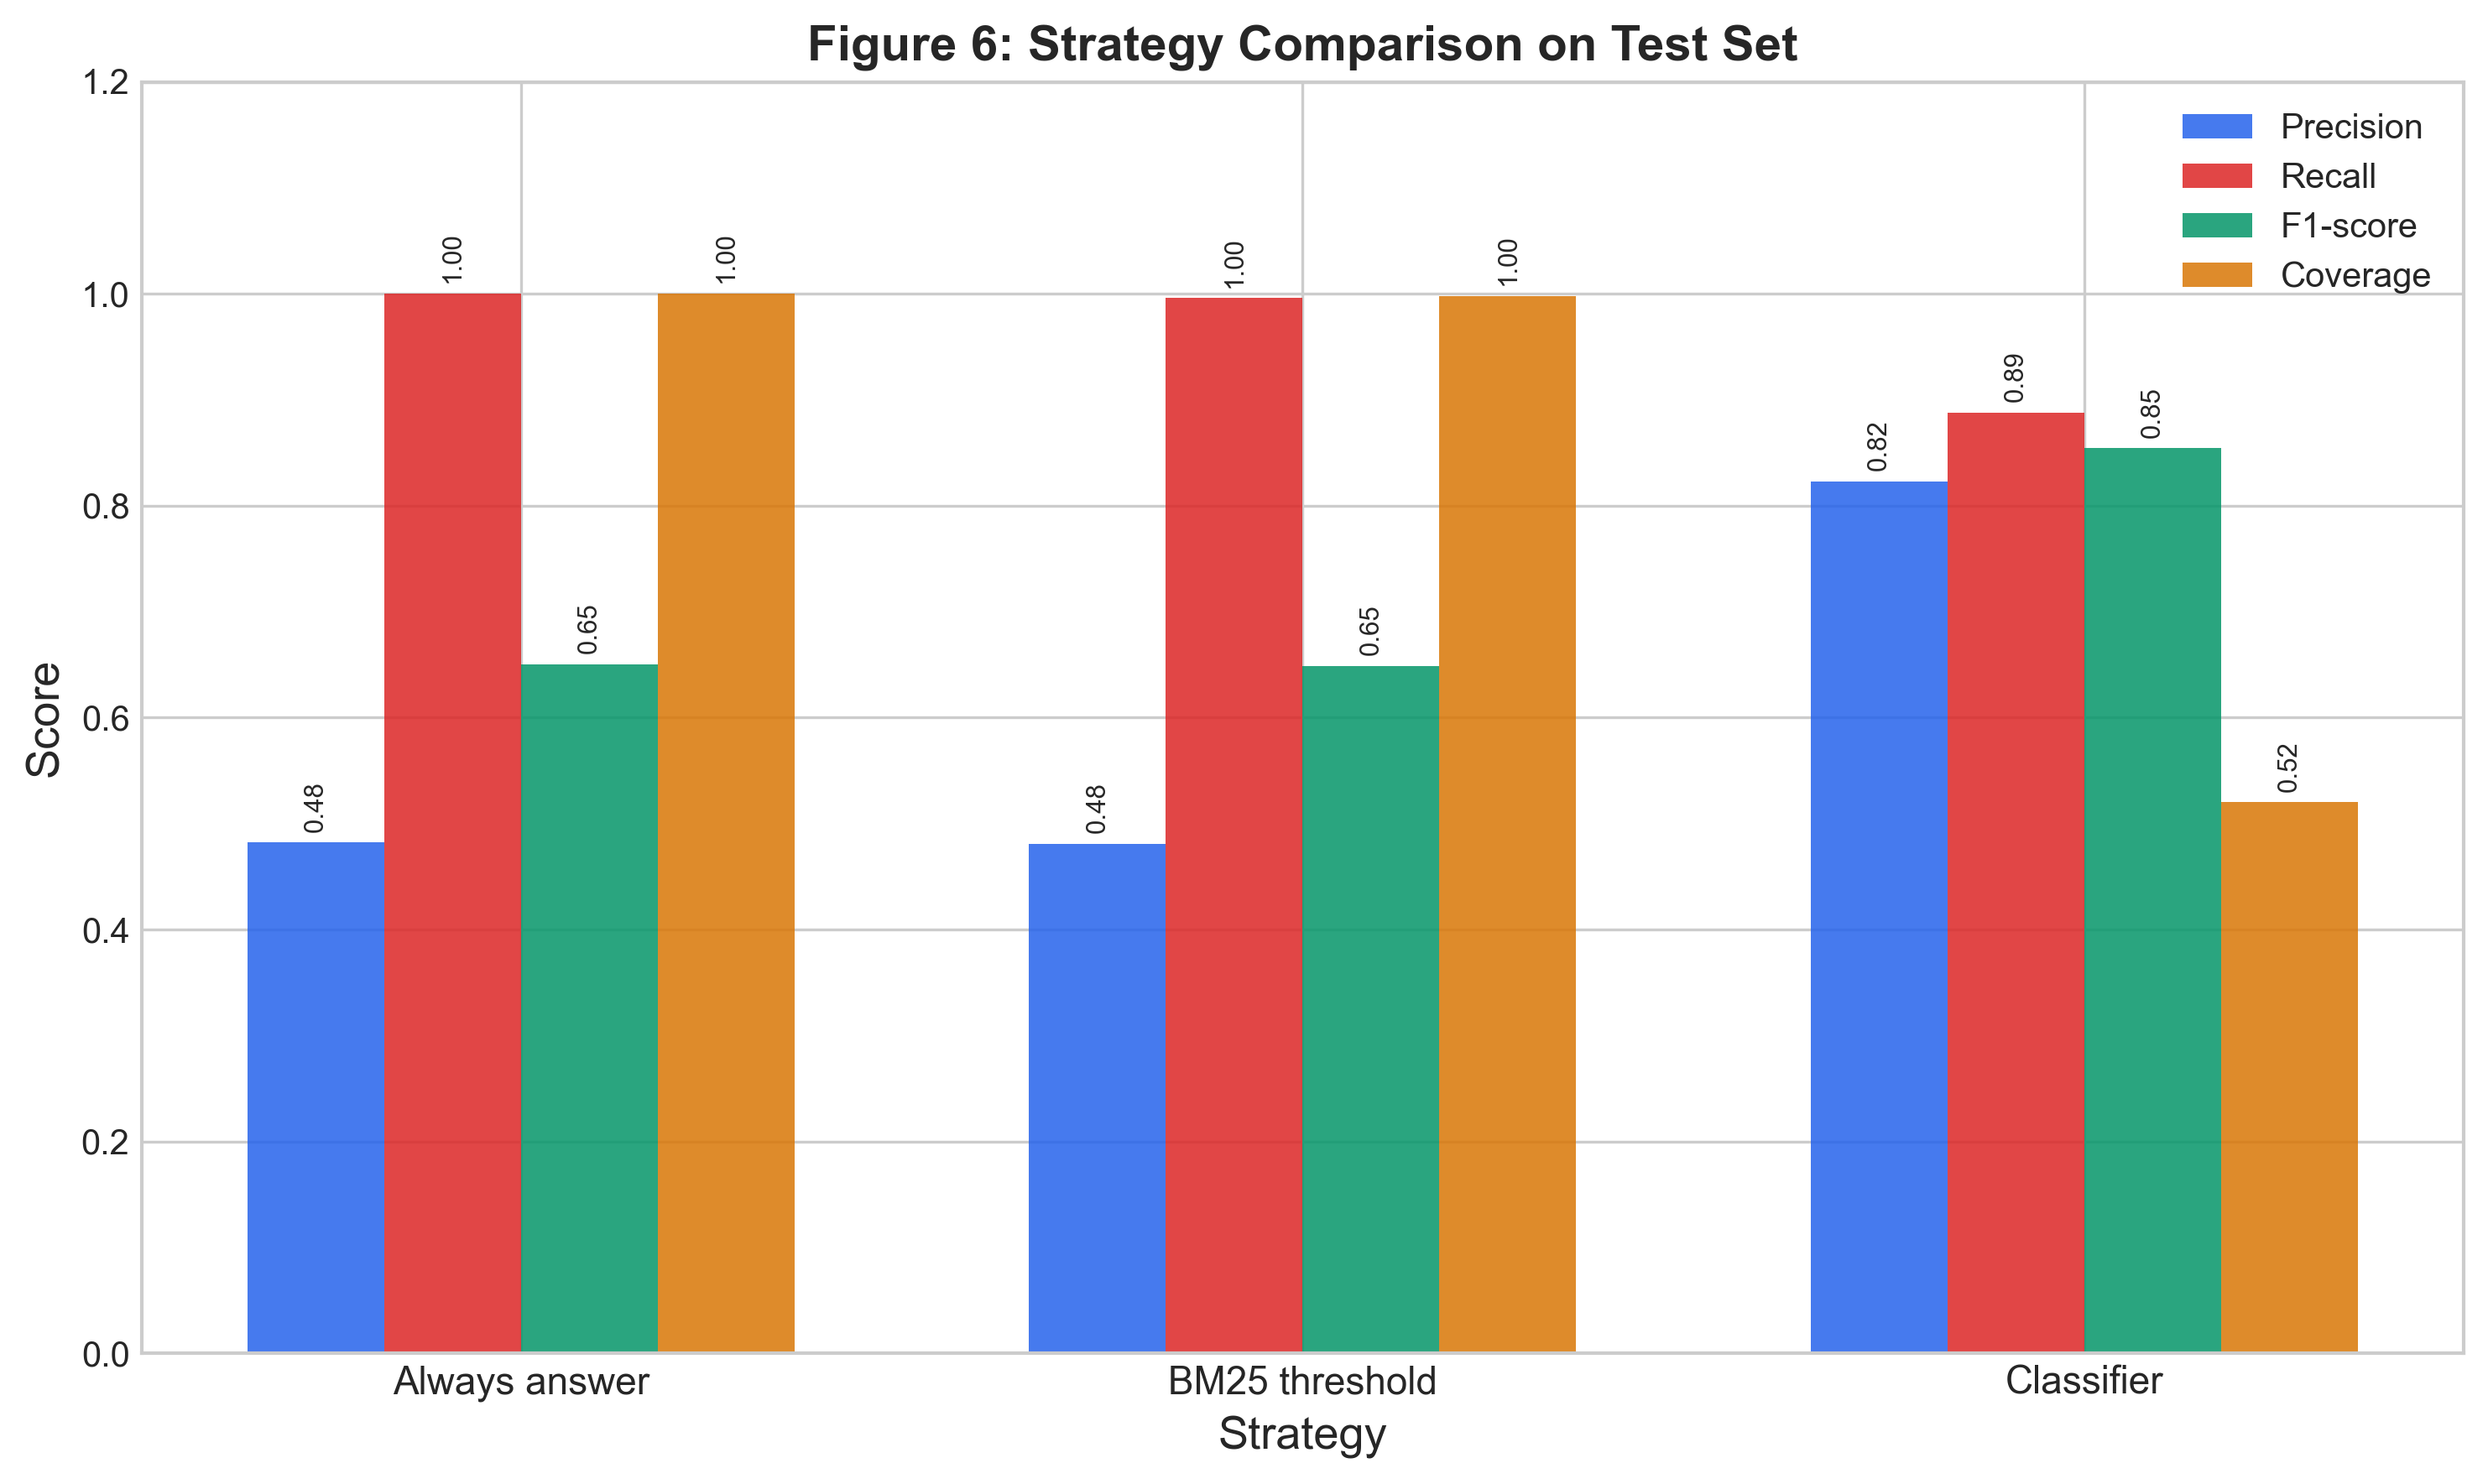
\includegraphics[width=0.80\textwidth]{fig6_strategy_comparison}
  \caption{Grouped bar chart comparing Precision, Recall, F1 and Coverage
           across the three abstention strategies on the test set.}
  \label{fig:strategy_comparison}
\end{figure}

\section{Interpretation}
\label{sec:results_interpretation}

\paragraph{Always Answer (Baseline).}
By design, this strategy achieves perfect recall ($= 1.00$) and perfect
coverage ($= 1.00$), since it never abstains. However, its precision is only
0.4820—barely above the random 50\% baseline on a balanced dataset—and its
False-Answer Rate is 1.00, meaning it provides a spurious answer to every
unanswerable question. The resulting F1 of 0.6505 reflects the fundamental
tension: high coverage is purchased at the cost of extreme imprecision on
unanswerable questions.

\paragraph{BM25 Threshold.}
The BM25 Threshold strategy (optimal validation-tuned $\tau$) achieves nearly
identical metrics to the baseline: precision 0.4810, F1 0.6486, and
False-Answer Rate 1.00. Coverage falls marginally to 0.998, meaning only 2.4
questions out of 1,200 are suppressed (2 questions, in absolute terms). This
result is striking: a single BM25 score threshold is essentially \emph{unable}
to discriminate answerable from unanswerable questions at the score levels
produced by the retriever over this dataset. The near-identical performance to
the baseline suggests that \emph{BM25 score alone is a poor abstention signal}
when used as a simple threshold.

\paragraph{Answerability Classifier.}
The logistic regression classifier achieves substantially superior results:
precision 0.8231, recall 0.8880, and F1 0.8543. These are improvements of
+34.1 pp in precision and +19.4 pp in F1 over the best single-threshold
strategy. The False-Answer Rate drops dramatically from 1.00 to 0.1776,
meaning the system now correctly abstains on approximately 82\% of unanswerable
questions.

The cost is a reduced coverage of 0.520: the classifier chooses to answer
only 52\% of questions (624 out of 1,200), and of those it abstains on, 11.2\%
are actually answerable (False-Abstention Rate = 0.1120). Whether this
precision–coverage trade-off is acceptable depends on the deployment context:
in high-stakes settings, a 82\% reduction in false answers at the cost of
answering only half of questions is likely worthwhile.

\section{Threshold Selection}
\label{sec:results_threshold}

Figure~\ref{fig:threshold_selection} shows precision, recall, and F1 as
functions of the classifier probability threshold $\delta$ on the validation
set. The optimal threshold $\delta^* = 0.28$ lies well below 0.5, reflecting
the fact that the classifier's default operating point (argmax) is biased
toward answering, and a lower threshold is needed to push recall at the cost of
precision.

\begin{figure}[htbp]
  \centering
  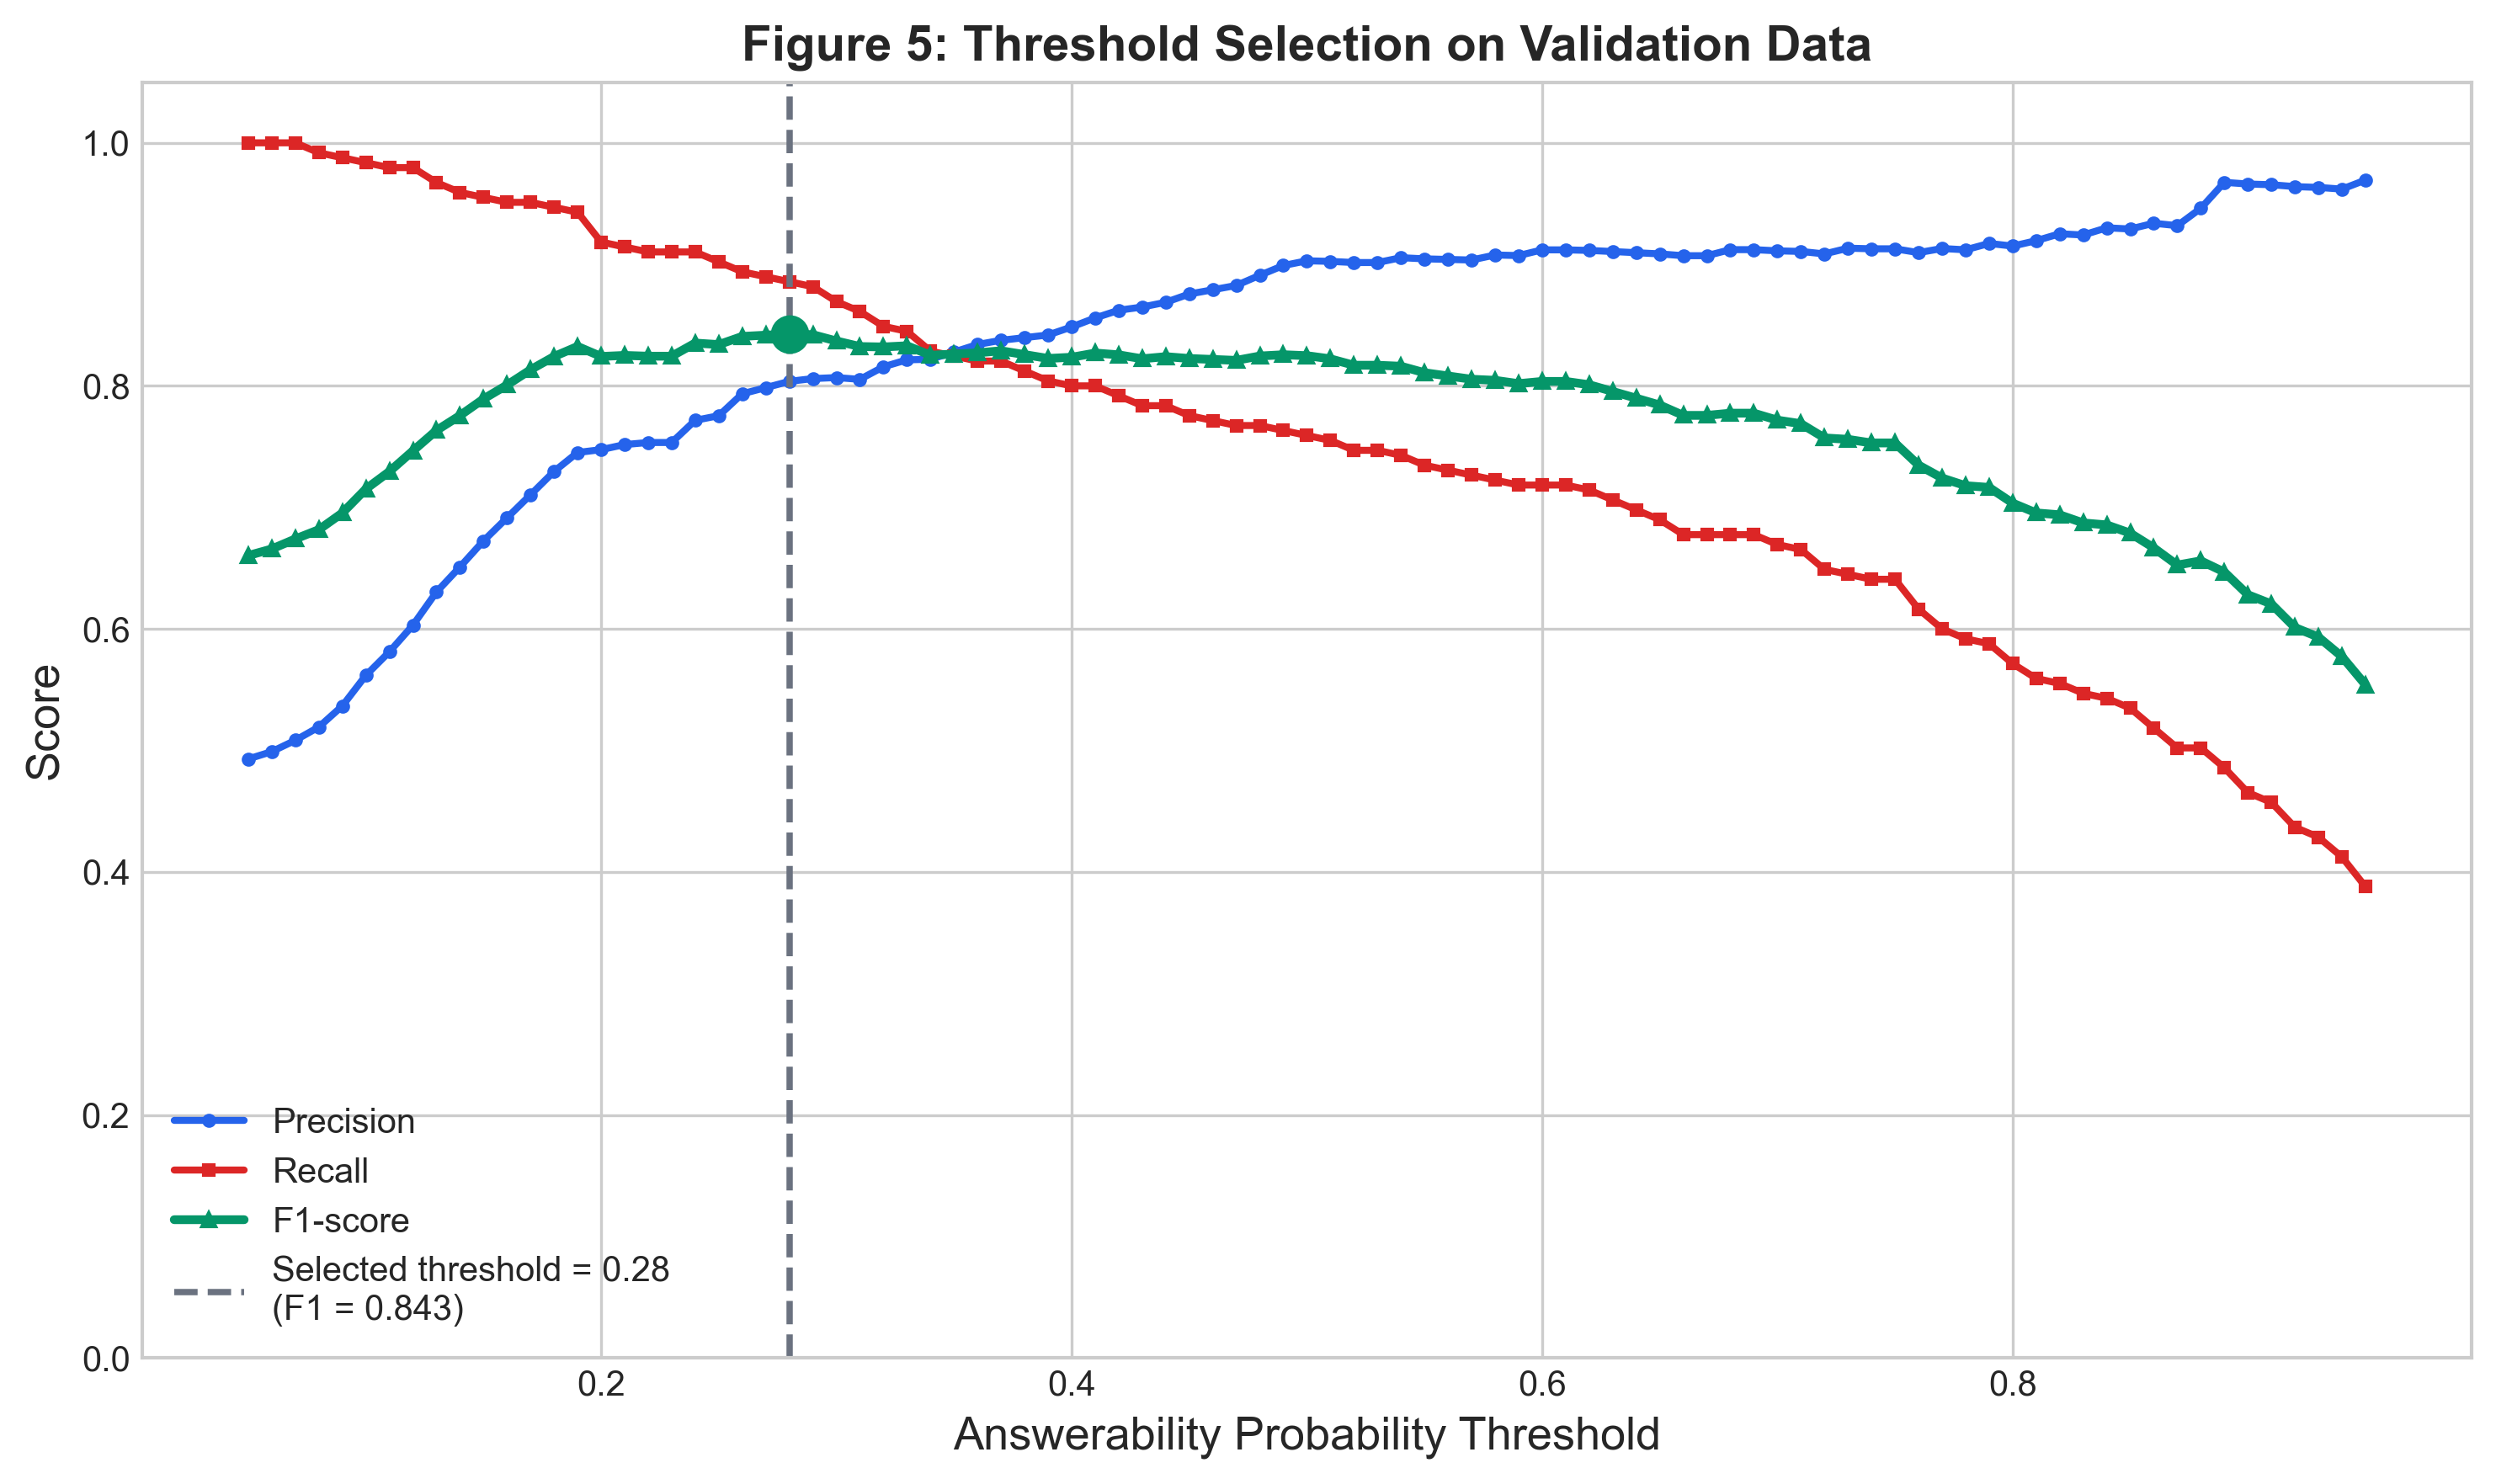
\includegraphics[width=0.80\textwidth]{fig5_threshold_selection}
  \caption{Precision, Recall, and F1 as functions of the classifier probability
           threshold on the validation set. The vertical dashed line marks the
           selected threshold $\delta^* = 0.28$.}
  \label{fig:threshold_selection}
\end{figure}

\section{Classifier Performance}
\label{sec:results_classifier}

Table~\ref{tab:classifier_performance} reports the classifier's binary
answerability prediction performance on the test set, treating the problem as
a binary classification task (answerable vs.\ unanswerable). The applied
threshold is $\delta^* = 0.28$.

\begin{table}[htbp]
  \centering
  \caption{Answerability classifier performance on the test set
           at threshold $\delta^* = 0.28$.}
  \label{tab:classifier_performance}
  \begin{tabular}{lcccc}
    \toprule
    \textbf{Set} & \textbf{Precision} & \textbf{Recall} & \textbf{F1} & \textbf{Accuracy} \\
    \midrule
    Test  & 0.8231 & 0.8880 & 0.8543 & 0.8540 \\
    \bottomrule
  \end{tabular}
\end{table}

\subsection{Confusion Matrix}

Figure~\ref{fig:confusion_matrix} and Table~\ref{tab:confusion_matrix} show the
confusion matrix on the test set.

\begin{table}[htbp]
  \centering
  \caption{Classifier confusion matrix on the test set.}
  \label{tab:confusion_matrix}
  \begin{tabular}{lcc}
    \toprule
    & \textbf{Predicted: Abstain} & \textbf{Predicted: Answer} \\
    \midrule
    \textbf{Actual: Unanswerable} & 213 (TN) & 46 (FP) \\
    \textbf{Actual: Answerable}   &  27 (FN) & 214 (TP) \\
    \bottomrule
  \end{tabular}
\end{table}

\begin{figure}[htbp]
  \centering
  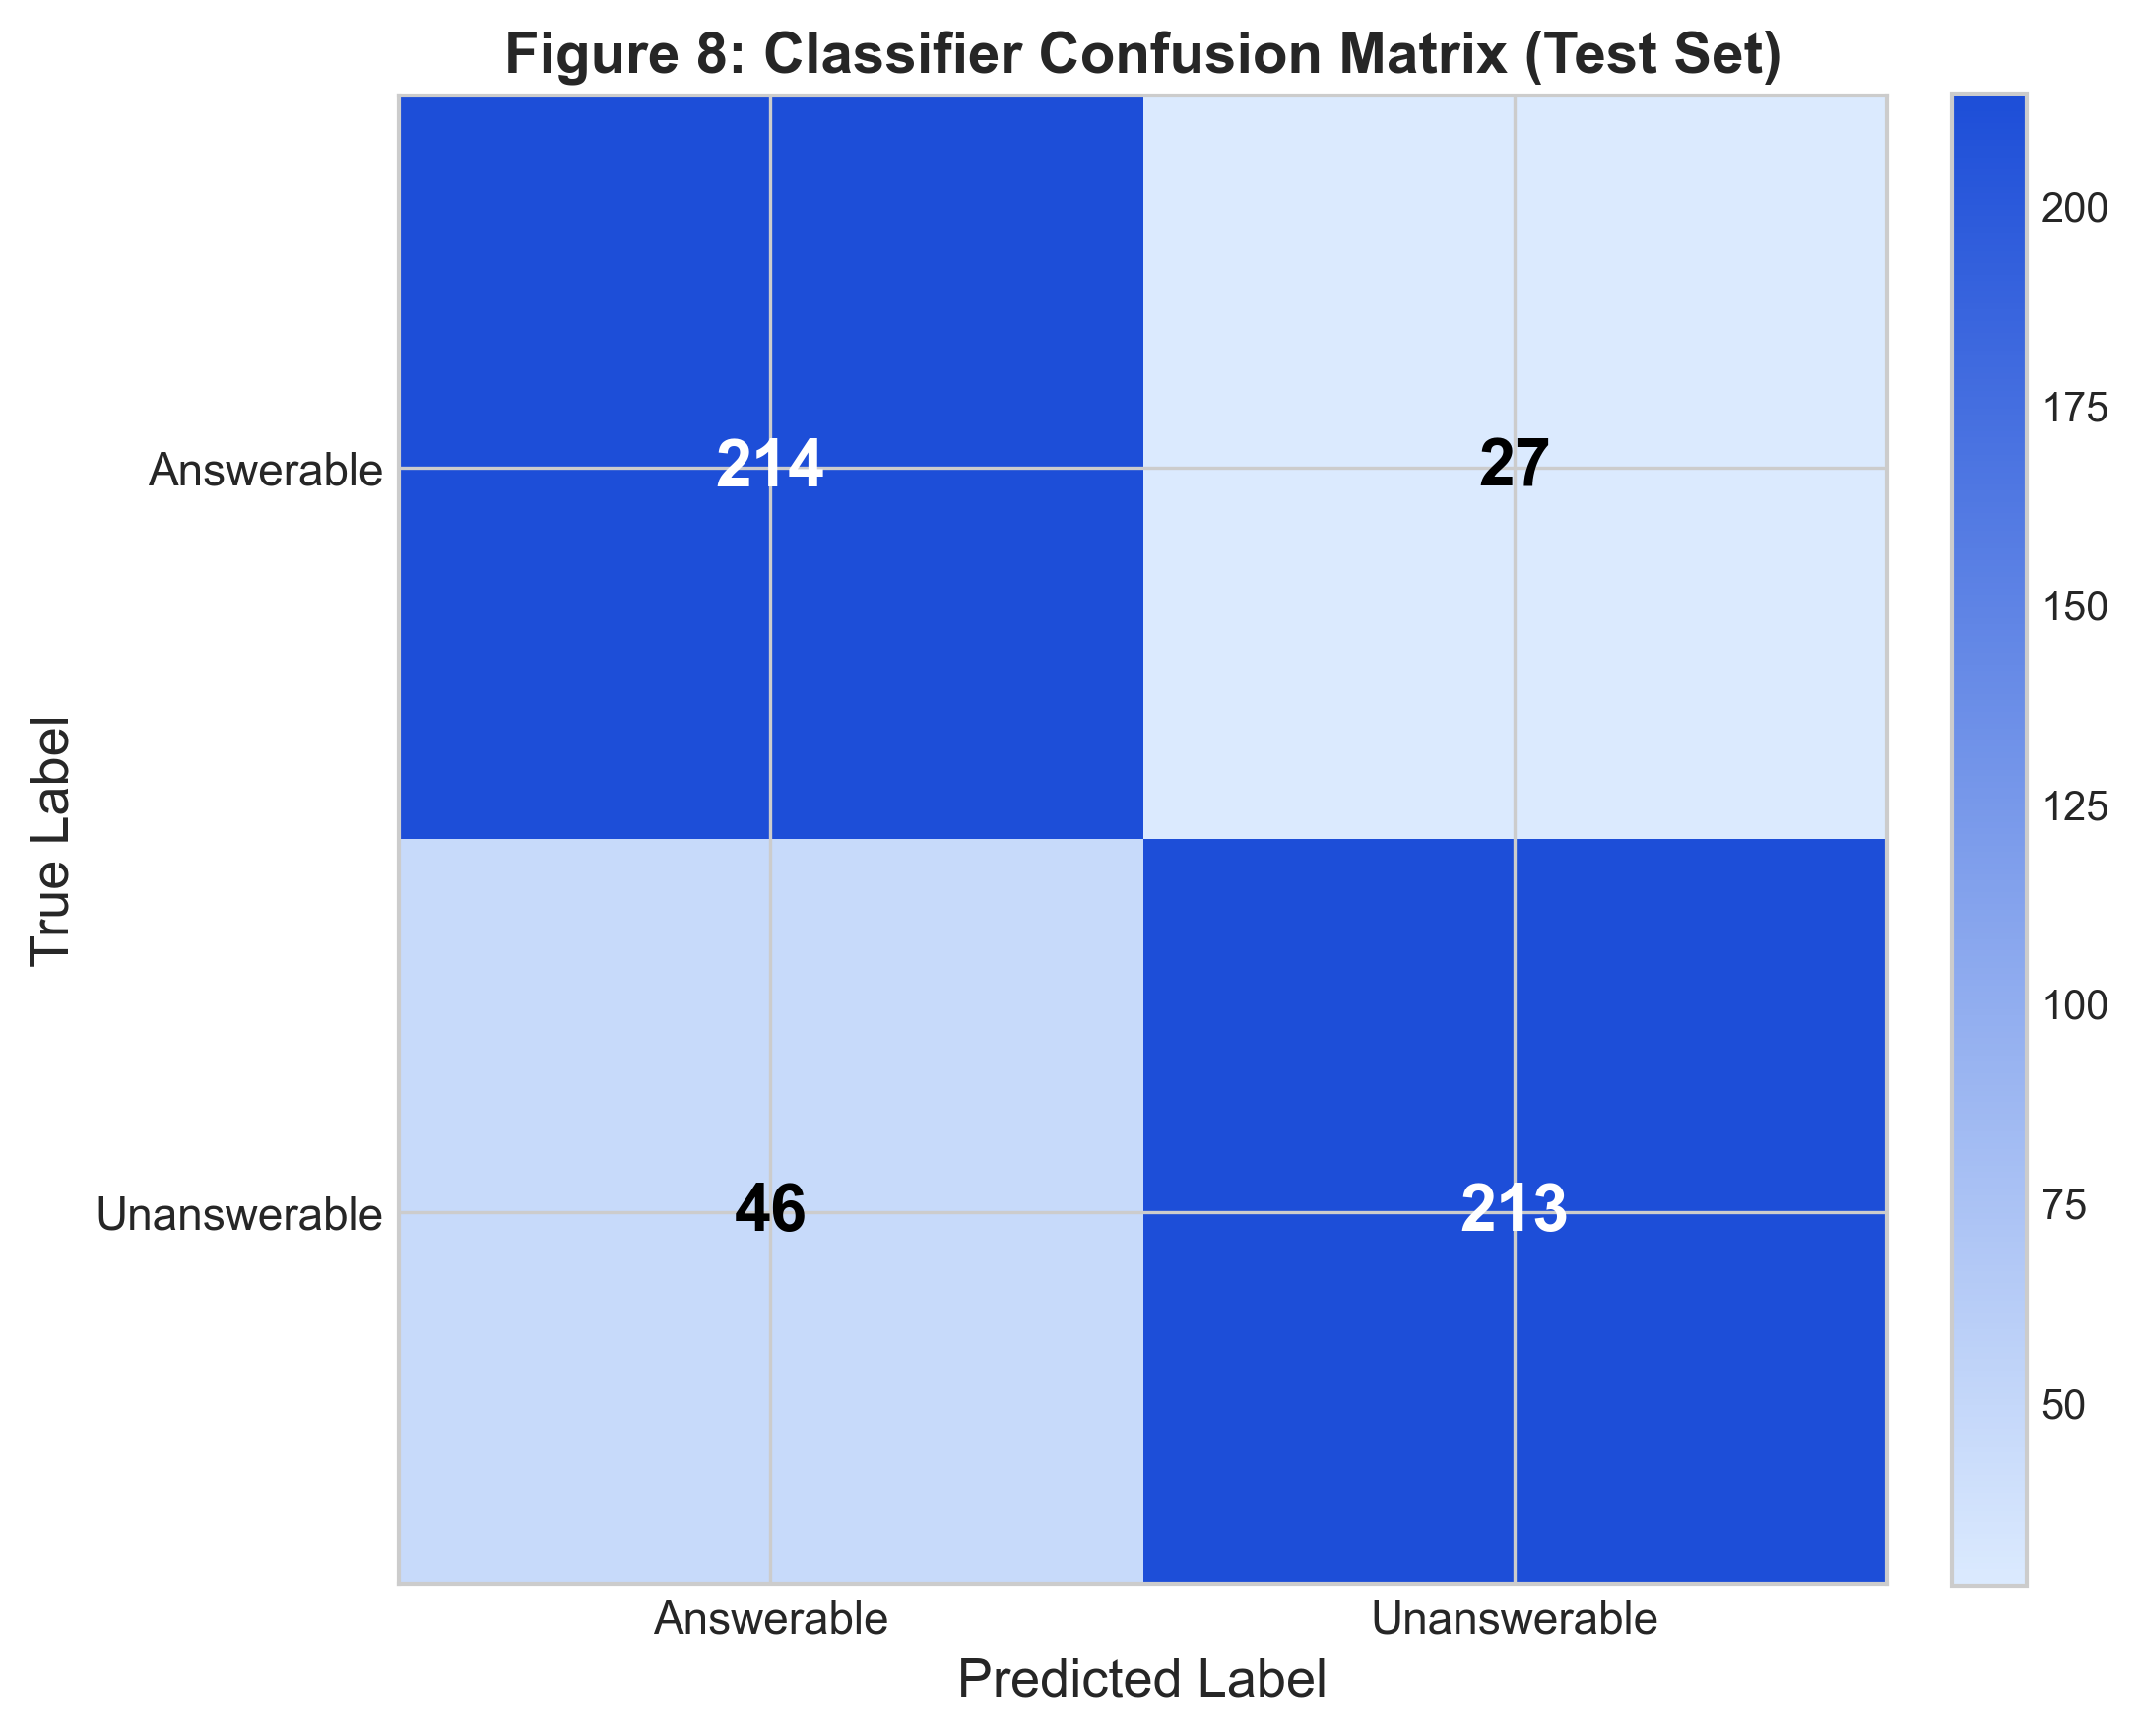
\includegraphics[width=0.60\textwidth]{fig8_confusion_matrix}
  \caption{Confusion matrix of the answerability classifier on the test set.
           TN = True Negative (correctly abstained), FP = False Positive (answered
           an unanswerable question), FN = False Negative (abstained on an
           answerable question), TP = True Positive (correctly answered).}
  \label{fig:confusion_matrix}
\end{figure}

The confusion matrix reveals an asymmetry: the classifier makes
$\text{FP} = 46$ errors (answering unanswerable questions) compared to
$\text{FN} = 27$ errors (abstaining on answerable ones). Given the threshold
$\delta^* = 0.28 < 0.5$, this is expected: the classifier is biased toward
answering, as false abstentions (FN) are penalised more under the F1 objective
used for threshold selection.

\section{Error Analysis Figures}
\label{sec:results_error_fig}

Figure~\ref{fig:error_analysis} shows the breakdown of correct answers,
correct abstentions, false answers, and false abstentions for each strategy,
providing an intuitive comparison of error profiles.

\begin{figure}[htbp]
  \centering
  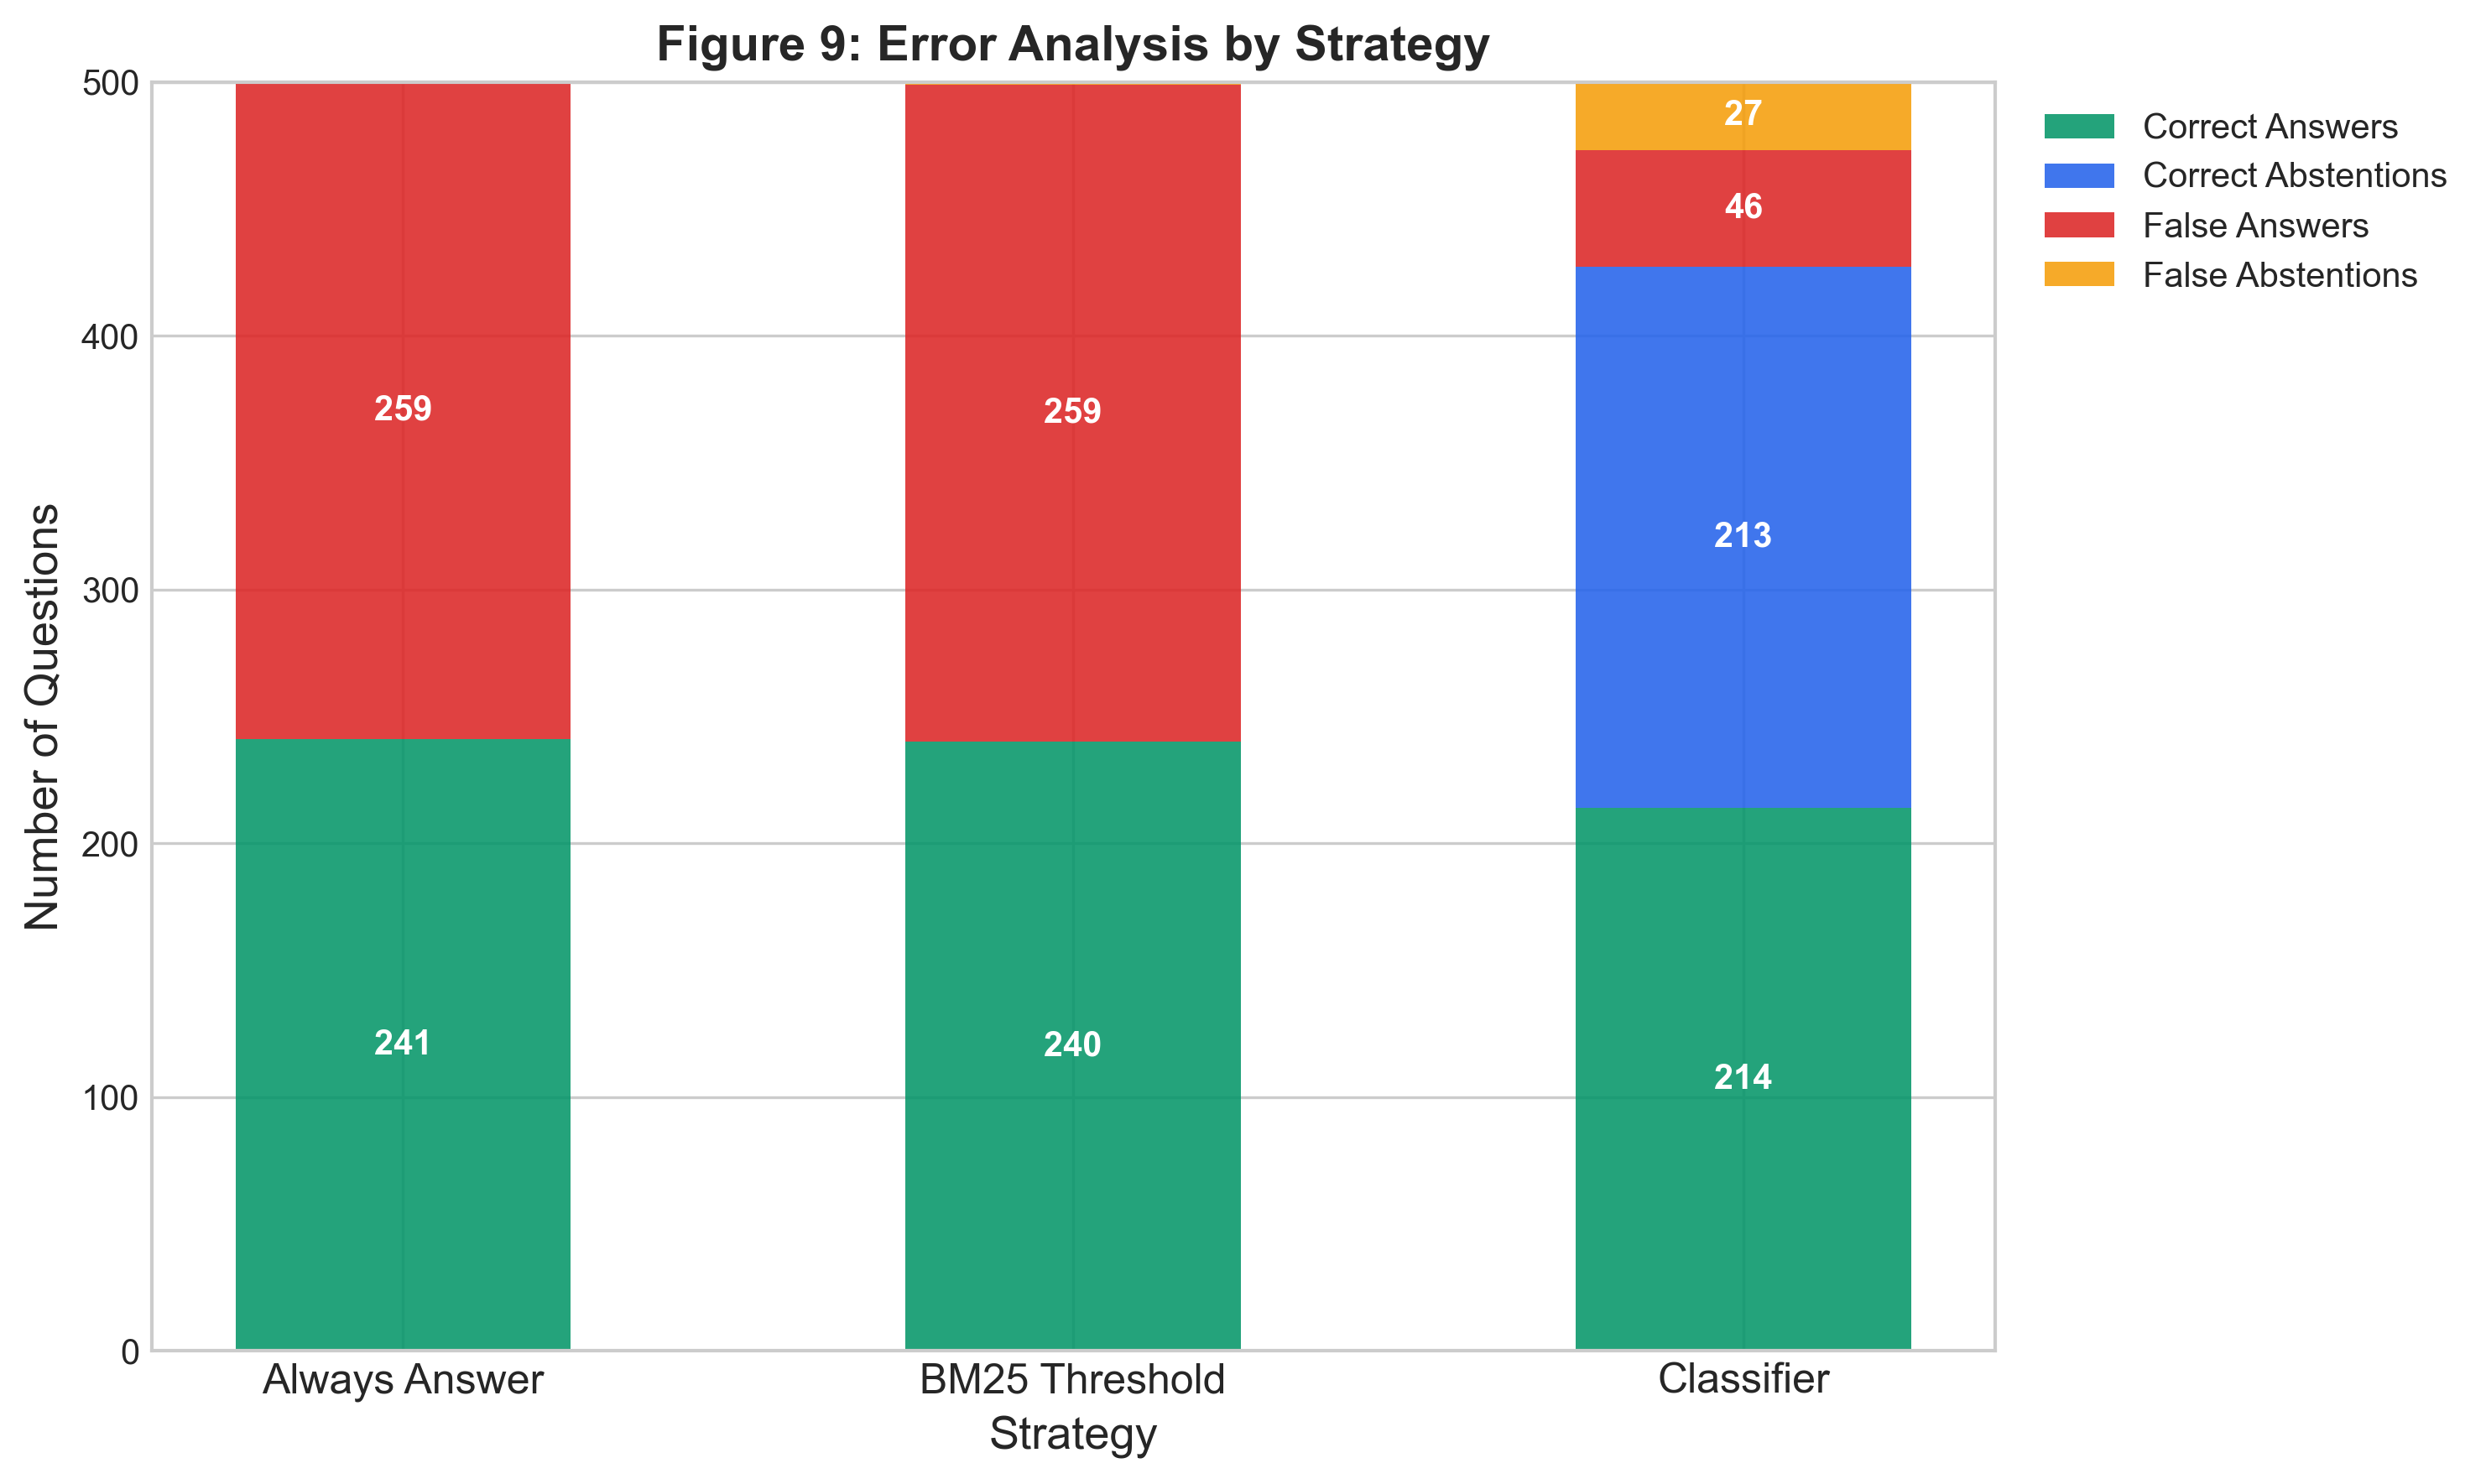
\includegraphics[width=0.80\textwidth]{fig9_error_analysis}
  \caption{Per-strategy breakdown of outcome types on the test set:
           Correct Answer, Correct Abstention, False Answer (answered when should
           have abstained), and False Abstention (abstained when should have
           answered).}
  \label{fig:error_analysis}
\end{figure}
